\section{Plant ROM Modeling}
\label{sec:plantRomModeling}

\newcommand{\DPM}[1]{\textcolor{magenta}{#1}}

For the six plant models considered in this analysis, we have chosen to use
$k$-nearest neighbor classifiers as surrogates to predict the presence
of core damage in each of the models.
%
Each surrogate is trained on a separate set of Monte Carlo samples, and
cross-validated using 3-fold validation in order to select an optimal value for
$k$.
%
In 3-fold validation, the data is split into three subsets and trained on two
of the subsets where the third subset is used to evaluate the prediction
accuracy.
%
The $k$-value that fits the data with the highest accuracy is considered the
``best'' parameter setting.
%
We repeat this process ten times for each model to ensure stability of the
results using multiples of 5 up to 50 for values of $k$ ($5,10,15,20,25,30,35,40,45,50$).

We evaluate the convergence of each rom by evaluating the mean and standard
deviation of the prediction accuracy over various training sizes, where a subset
of the training data is used to construct a surrogate which is then used to
predict on the entire validation set.
%
An example of this convergence is shown in Figure~\ref{fig:romConvergence}.
%
\DPM{Expand...}
%
The resulting $k$ values used for each model are reported in Table~\ref{tab:romInfo}.
\DPM{Figure~\ref{fig:neighborSelection}}

\begin{table}[!htbp]
	\centering
	\begin{tabular}{ l | c | c | c | c | c }
	      & \textbf{Parameter} & \textbf{Optimal} & \textbf{Training} & \textbf{Validation} & \textbf{Prediction} \\
	\textbf{Model} & \textbf{Count}     &   \textbf{$k$}   &   \textbf{size}   &    \textbf{size}    &  \textbf{accuracy (\%)} \\
	\hline
	\hline
	PWR1 &  7 &  5 &  4596 & 2500 & 100.0 \\
	% \hline
	PWR2 &  3 & 25 &  4951 &  439 & 99.32 \\
	% \hline
	PWR3 & 10 & 50 & 12000 & 3990 & 100.0\\
	% \hline
	SFP1 &  3 &  5 &  2883 & 2876 & 99.72 \\
	% \hline
	SFP2 &  5 &  5 &  4695 & 4714 & 99.02 \\
	% \hline
	SFP3 &  3 &  5 &  2807 & 2817 & 99.04 \\
	\end{tabular}
	 \caption{Surrogate model settings and validation information.}
	 \label{tab:romInfo}
\end{table}

\begin{figure}[!htbp]
	\centering
	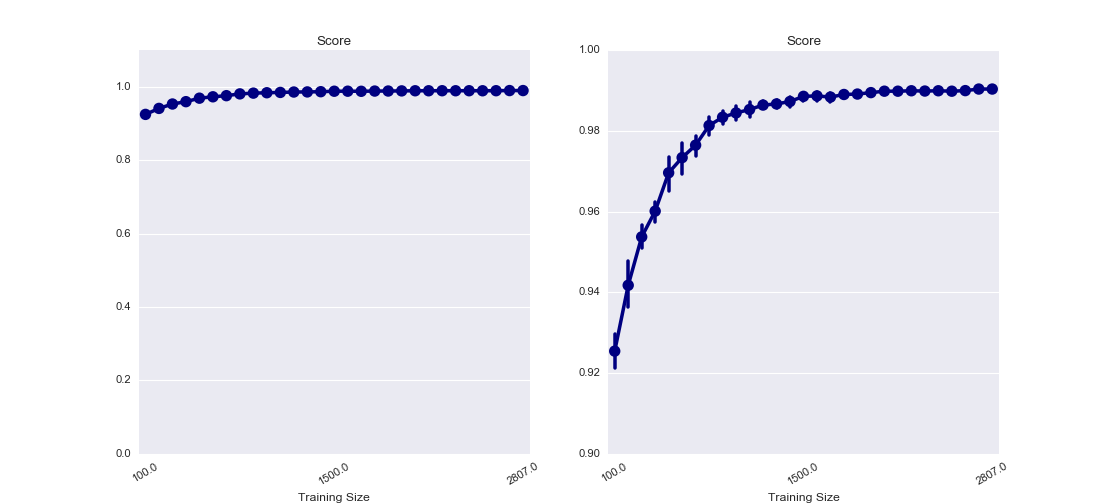
\includegraphics[width=0.98\textwidth]{convergenceSFP3.png}
	\caption{Convergence of the Prediction Accuracy with increasing sample sizes. Each data point is the average of ten trials
	worth of data with error bars representing one standard deviation.}
	\label{fig:romConvergence}
\end{figure}

\begin{figure}[!htbp]
	\centering
	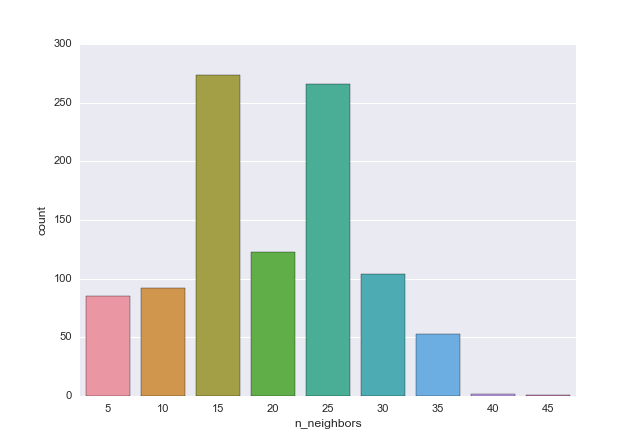
\includegraphics[width=0.98\textwidth]{neighborCVPWR2.png}
	\caption{Histogram of the ``best'' $k$ value for the PWR2 model when trained on 1000 variations of size 2475 drawn from a pool of 4951 training samples. \DPM{Use other figure here where k=25 was better than k=15.}}
	\label{fig:neighborSelection}
\end{figure}